\documentclass[11pt,border=4pt]{standalone}
\usepackage{amsmath,amssymb,bm,mathtools}
\usepackage[fontset=fandol]{ctex}
\usepackage{tikz}
\usetikzlibrary{arrows.meta,calc,patterns,angles,quotes,decorations.markings,decorations.pathmorphing}
\newcommand{\dd}{\mathop{}\!\mathrm d}
\newcommand{\e}{\mathrm e}
\tikzset{axis/.style={->,>=Stealth,line width=.45pt},world/.style={line width=.8pt},flow/.style={->,>=Stealth,line width=.7pt},ray/.style={->,>=Stealth,line width=.7pt},guide/.style={dashed,line width=.35pt},aux/.style={dashed,line width=.35pt},dim/.style={<->,>=Stealth,line width=.35pt},every node/.style={font=\small},force/.style={->,>=Stealth,very thick},gas/.style={fill=blue!7}}
\begin{document}
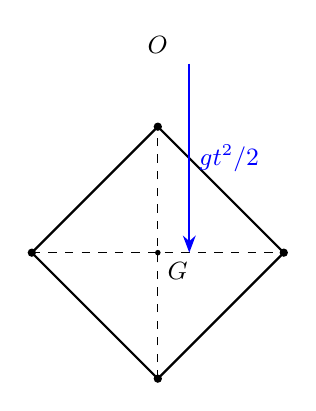
\begin{tikzpicture}\coordinate(G)at(0,0);\draw[world](0,1.6)--(1.6,0)--(0,-1.6)--(-1.6,0)--cycle;\foreach \p in {(0,1.6),(1.6,0),(0,-1.6),(-1.6,0)}\fill\p circle(1.5pt);\draw[guide](-1.6,0)--(1.6,0) (0,-1.6)--(0,1.6);\fill(0,0)circle(1pt)node[below right]{$G$};\node[above]at(0,2.4){$O$};\draw[flow,blue](.4,2.4)--(.4,0)node[midway,right]{$gt^2/2$};\end{tikzpicture}
\end{document}
